% !Mode:: "TeX:UTF-8"
\chapter{系统设计与实现}

本章介绍本文所构建的AutoChip风格RTL自动生成与反馈修复原型系统的总体架构、核心模块设计与关键实现细节。该系统以"生成—编译—仿真—反馈—修复"为核心闭环，支持多种benchmark接入、多模型切换、多种反馈策略与提示词策略，为后续实验提供了统一的可复现实验平台。

\section{系统总体架构}

\subsection{设计目标}

本系统的核心目标是构建一个可扩展、可审计的AutoChip风格实验平台\cite{autochip}，具体包括：接入多种公开RTL benchmark，将不同格式的题目统一为内部Task表示；调用大语言模型生成Verilog代码，并通过EDA工具链进行编译与仿真验证；将验证结果以结构化反馈形式返回模型，驱动迭代修复；记录完整实验过程元数据，确保结果可追溯、可审计。

\subsection{模块划分}

系统由以下核心模块组成：任务加载器（Task Loader）负责从不同benchmark目录中读取题目描述、模块接口与测试平台文件，统一转化为内部Task数据结构；提示词构建器（Prompt Builder）根据任务描述、模块接口及可选的反馈信息，构建发送给大语言模型的提示词；大语言模型客户端（LLM Client）封装API调用逻辑，通过第三方统一网关接入多种模型；Verilog提取器从模型返回的文本中提取代码块；Verilog执行器调用Icarus Verilog编译器和VVP仿真器；评分器基于编译与仿真结果对候选代码打分；反馈循环控制器实现完整的迭代闭环；实验产物管理器负责元数据记录与结果序列化。

\begin{figure}[htbp]
\centering
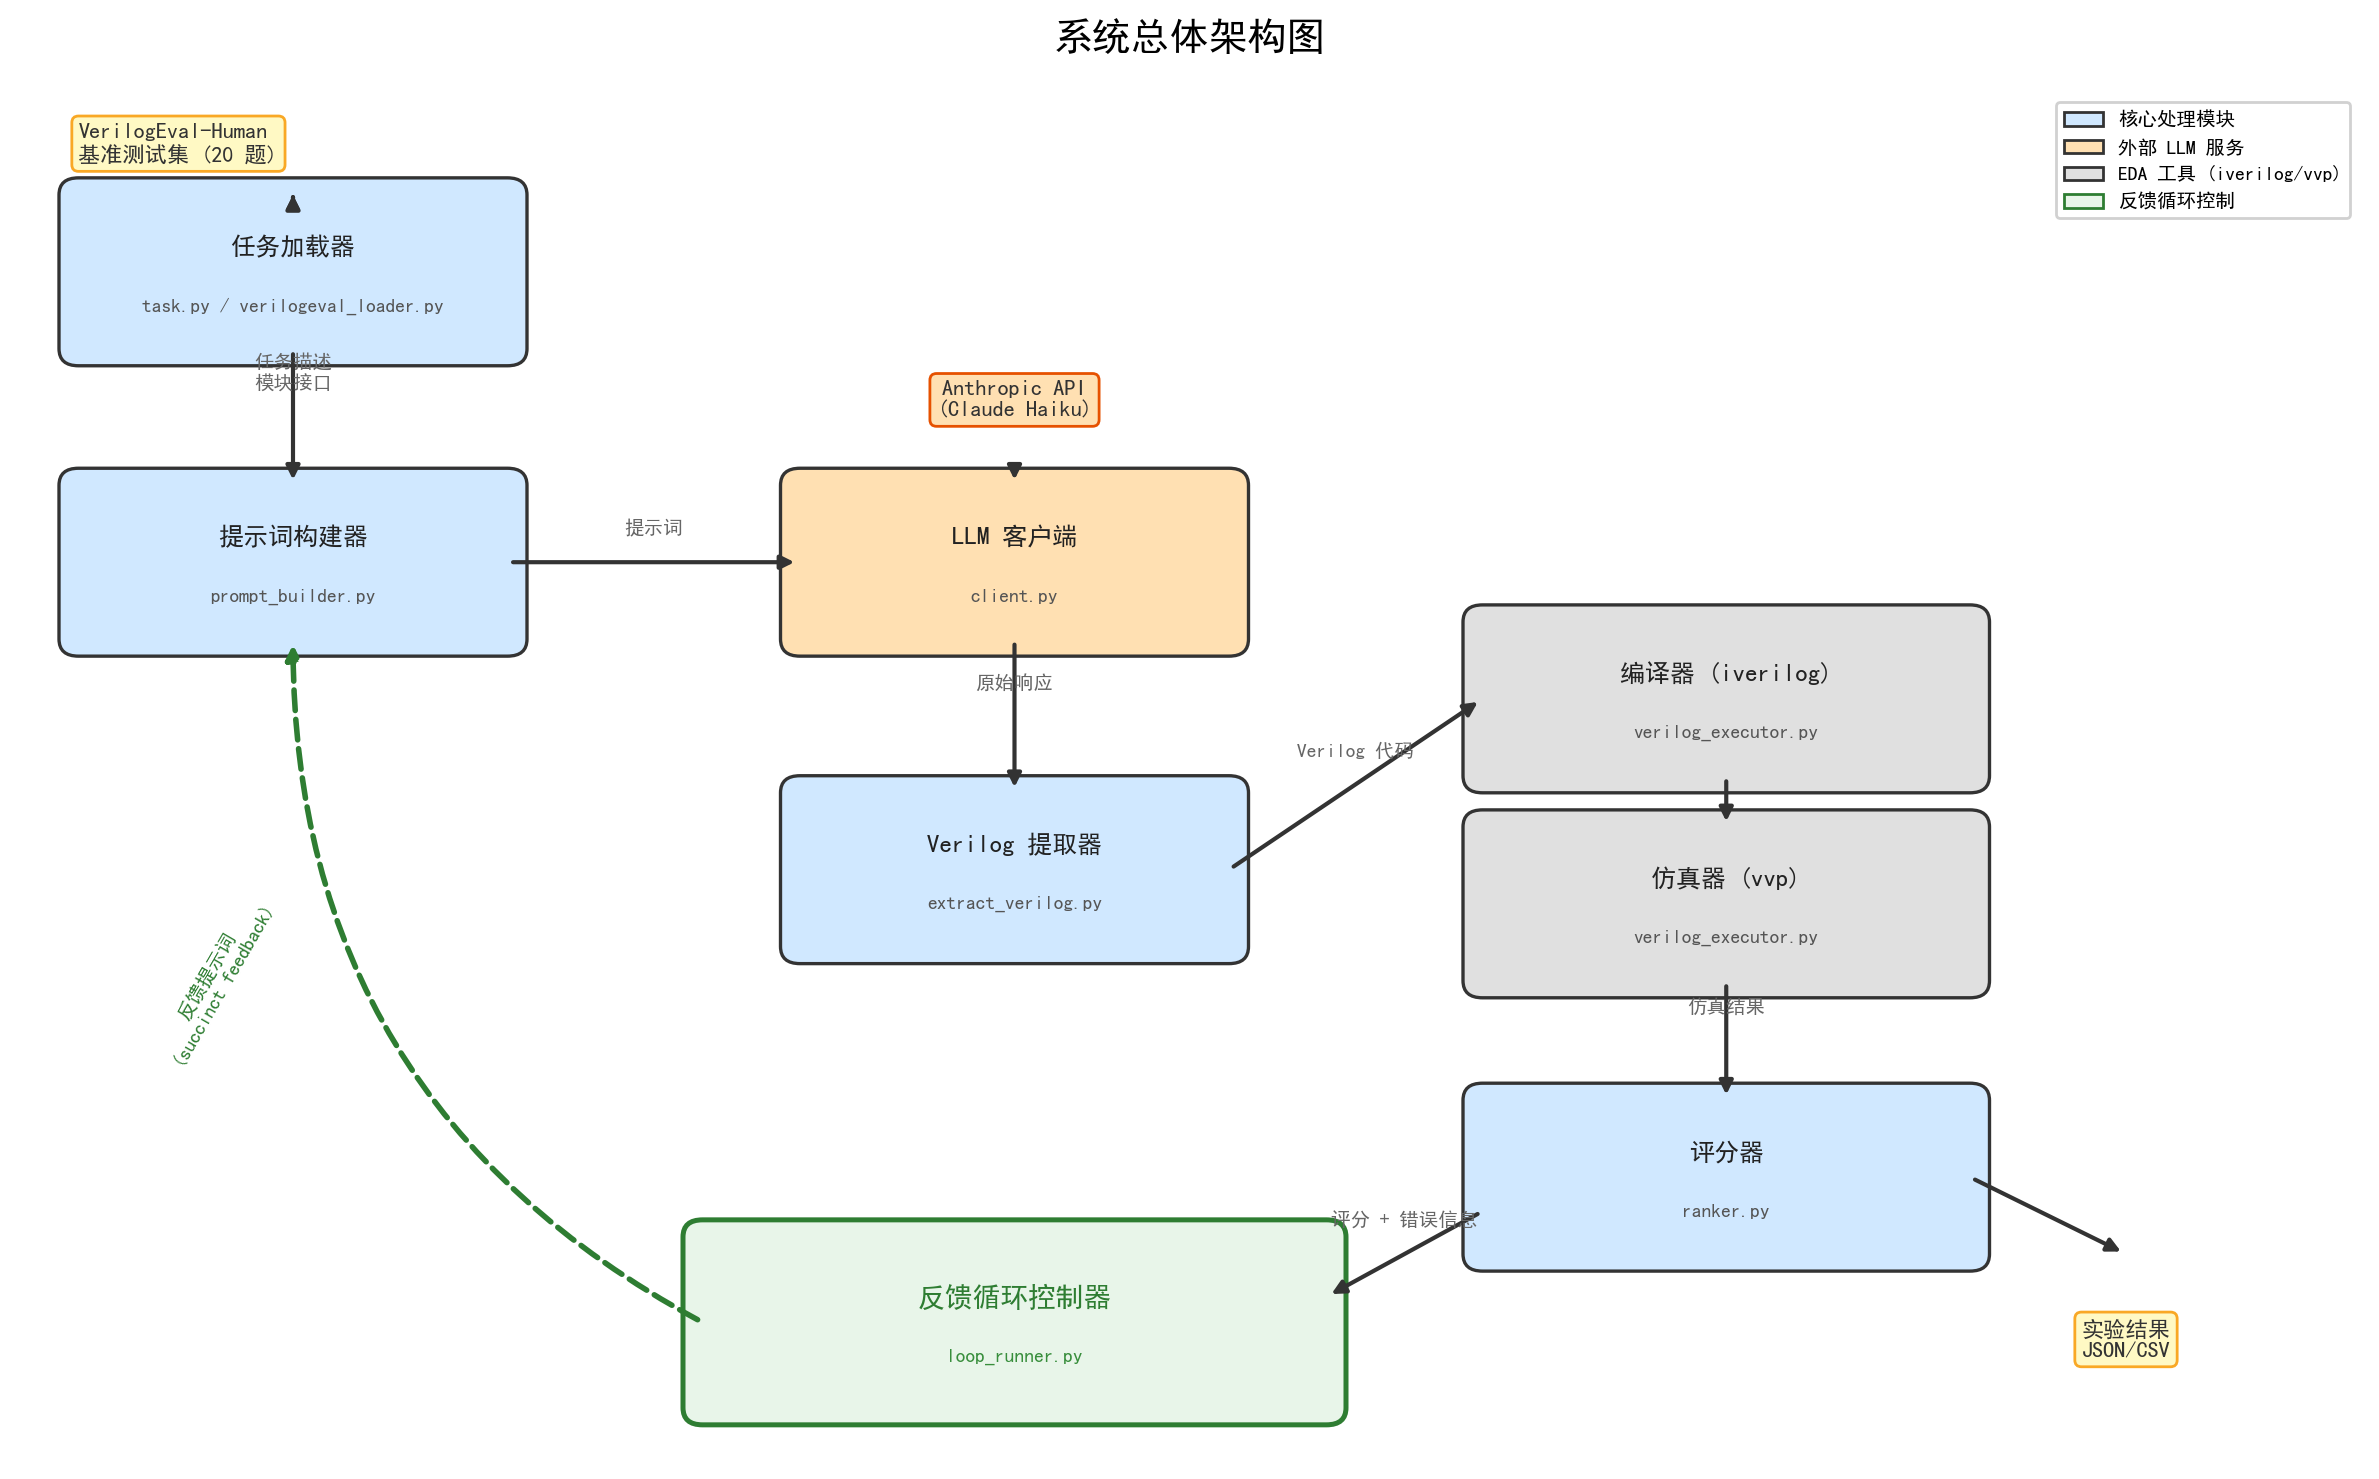
\includegraphics[width=0.9\textwidth]{figure/fig_system_architecture.png}
\caption{AutoChip风格RTL生成与反馈修复系统架构}
\label{fig:system_architecture}
\end{figure}

图\ref{fig:system_architecture}展示了系统的整体数据流：任务加载器从benchmark目录读取题目，提示词构建器将题目描述与反馈信息组织为提示词，LLM客户端调用模型获得自然语言回复，Verilog提取器从中提取代码，执行器进行编译与仿真，评分器给出分数，反馈循环控制器根据分数决定是否继续迭代。

\section{任务加载与Benchmark接入}

\subsection{Task数据结构}

为了屏蔽不同benchmark在文件组织和题目格式上的差异，系统定义了统一的Task数据结构，包含四个核心字段：任务名称（name）、自然语言描述（description）、模块接口声明（module\_header）以及测试平台文件路径（testbench\_path）。

\subsection{VerilogEval-Human加载器}

VerilogEval\cite{verilogeval}采用spec-to-RTL模式，提供自然语言描述和TopModule接口定义。VerilogEval加载器的核心逻辑是：读取自然语言描述作为description，读取接口声明作为module\_header，将参考实现与测试平台合并后写入临时文件作为testbench\_path。

\subsection{RTLLM加载器}

RTLLM\cite{rtllm}的每个题目目录包含一个自然语言设计描述文件和一个独立的测试平台文件。RTLLM加载器通过递归遍历分类目录来发现所有题目，对每个包含\texttt{design\_description.txt}和\texttt{testbench.v}的目录创建一个RTLLMProblem对象。

\subsection{适配层的必要性}

两个benchmark在文件结构、描述格式、测试平台组织和仿真输出格式上的差异，使得专用加载器成为必要。统一的Task接口确保了反馈循环控制器和评分器等下游模块无需关心数据来源。

\section{大语言模型调用与模型管理}

\subsection{统一API网关架构}

本系统通过第三方统一API网关接入多种大语言模型。网关的核心价值在于：保持API密钥和服务端点固定不变，仅通过模型名称参数切换不同的底层模型。

\subsection{重试机制与错误分类}

系统内置了指数退避重试机制：对可重试的瞬态错误自动重试最多3次，退避间隔为2s、5s、10s。当所有重试均失败时，错误信息被封装为结构化的APIError对象，记录到该候选结果中。

\subsection{对实验可追溯性的意义}

上述设计确保了两个关键属性：任何实验结果都可以精确追溯到使用的模型名称和调用参数；API错误不会污染实验数据。

\section{Verilog代码提取、编译与仿真执行}

\subsection{代码提取}

Verilog提取器首先移除Markdown代码围栏标记，然后使用正则表达式匹配所有\texttt{module ... endmodule}结构。该设计对CoT提示策略具有兼容性。

\subsection{编译执行}

编译阶段使用Icarus Verilog\cite{iverilog}将生成的设计代码与测试平台一起编译，启用\texttt{-g2012}选项支持SystemVerilog 2012标准，并设置30秒超时保护。

\subsection{仿真执行与结果解析}

仿真阶段使用VVP执行编译产生的仿真二进制文件，设置60秒超时保护。解析器实现了双格式支持：VerilogEval格式匹配\texttt{mismatched samples is N out of M}模式；RTLLM格式匹配\texttt{Your Design Passed}或\texttt{Test completed with N/M failures}。

\subsection{评分机制}

评分器基于AutoChip论文定义的排序规则，将编译与仿真结果映射为一个标量分数，如表\ref{tab:rank_score}所示。

\begin{table}[htbp]
\centering
\caption{评分机制定义}
\label{tab:rank_score}
\begin{tabular}{lrl}
\toprule
情况 & 分数 & 含义 \\
\midrule
未提取到有效Verilog & $-2.0$ & 代码提取失败 \\
编译失败 & $-1.0$ & 存在语法或结构错误 \\
编译有警告但无仿真结果 & $-0.5$ & 可能存在问题 \\
编译成功但无仿真数据 & $0.0$ & 无法评估正确性 \\
仿真部分通过 & $0 \sim 1.0$ & (总样本$-$不匹配)/总样本 \\
仿真完全通过 & $1.0$ & 设计正确 \\
\bottomrule
\end{tabular}
\end{table}

\section{反馈循环控制机制}

反馈循环是本系统的核心，实现了AutoChip论文提出的"生成—验证—反馈—修复"迭代闭环。

\begin{figure}[htbp]
\centering
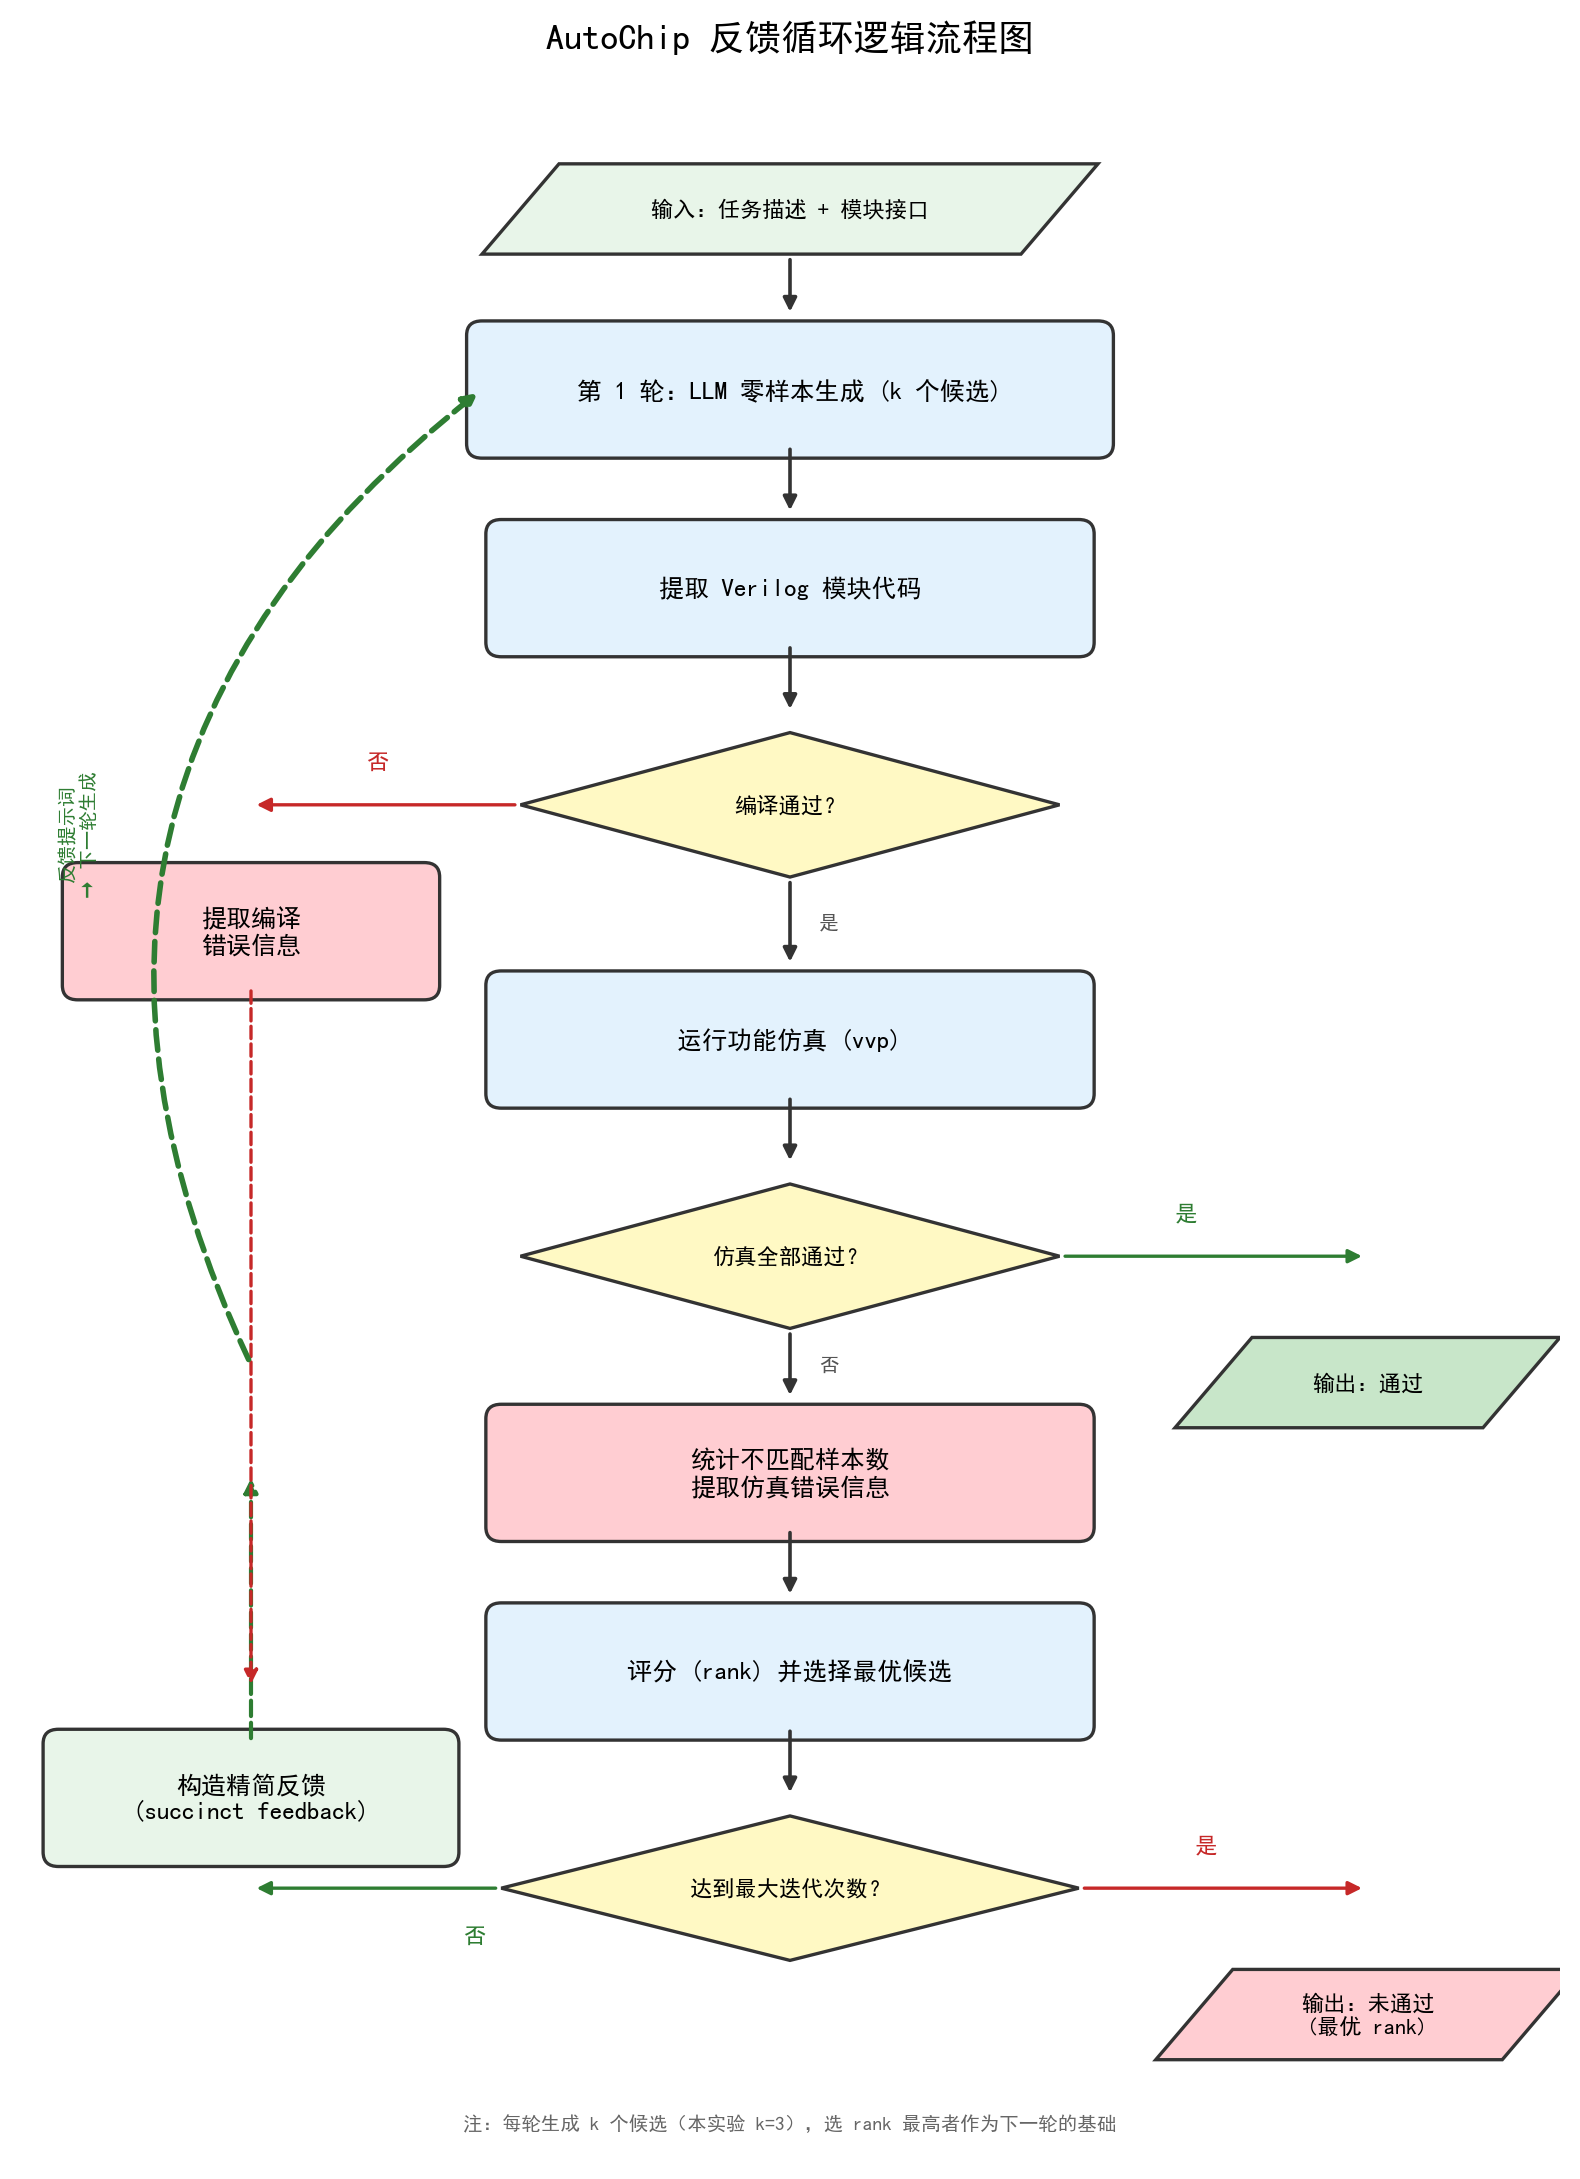
\includegraphics[width=0.85\textwidth]{figure/fig_feedback_loop_flow.png}
\caption{反馈循环控制流程}
\label{fig:feedback_loop}
\end{figure}

\subsection{单轮反馈循环}

单轮反馈循环（Single-turn Feedback Loop）的执行流程如下：第1轮使用初始提示词生成$k$个候选代码，分别编译、仿真、评分，选出全局最优候选；第2轮及后续，将全局最优候选的代码和对应的编译/仿真错误信息组织为反馈提示词，再次生成$k$个候选。循环直到某候选通过（rank$=$1.0）或达到最大迭代次数（默认5轮）。

全局最优追踪机制确保了反馈循环具有单调性。

\subsection{Zero-shot作为退化形式}

零样本模式可视为反馈循环的退化形式：$k=1$、max\_iterations$=$1。这一设计使得零样本基线实验和反馈实验共享相同的代码路径，确保了实验条件的公平性。

\subsection{Retry-only模式}

为了区分反馈循环中"多次重试"和"错误反馈信息"各自的贡献，系统实现了retry-only模式：在该模式下，所有迭代均使用初始提示词，不包含任何错误反馈信息。

\subsection{API错误处理}

当某个候选的API调用失败时，该候选被标记为api\_error但不终止整个迭代。只有当一轮迭代中所有$k$个候选全部因API错误而失败时，循环才提前终止。

\section{反馈策略扩展实现}

\subsection{反馈粒度级别}

为了研究反馈信息量对修复效果的影响，系统实现了三种反馈粒度级别：Level 2（Compile-only，仅编译反馈）仅反馈编译阶段的错误信息；Level 3（Succinct，简洁反馈）在编译反馈的基础上增加仿真失败时的不匹配样本数和仿真输出前40行，是系统的默认级别；Level 4（Rich，丰富反馈）进一步扩展仿真输出到前80行并添加显式分析提示。

结合loop\_runner中零样本（Level 0）和retry-only（Level 1），系统共支持五个梯度的反馈水平（L0--L4）。

\subsection{多轮对话反馈}

除单轮反馈外，系统还实现了多轮对话反馈模式（Multi-turn Feedback）。与单轮模式中每次API调用均为独立请求不同，多轮模式维护一个持续增长的对话历史。

多轮对话的关键设计考虑包括：初始消息使用简化版提示词；反馈消息不包含上一轮的代码（因为代码已存在于对话历史中）；反馈信息必须描述模型在对话中最后一轮生成的代码的错误，确保反馈与上下文一致。

\section{提示词策略扩展实现}

\subsection{四种提示策略}

为了研究初始提示词工程对RTL生成质量的影响，系统实现了四种可切换的提示策略\cite{cot,gpt3}：P0（Base Prompt，直接指令式提示）、P1（CoT Prompt，思维链提示）、P2（Few-shot Prompt，少样本提示）和P3（Few-shot + CoT Prompt）。

\subsection{数据泄漏防护}

Few-shot示例的选择需要避免数据泄漏。系统使用的两个示例——8位加法器和4位计数器——均不在正式实验使用的STUDY\_12子集中。

\subsection{策略调度机制}

提示策略通过PromptStrategy枚举类型定义，由实验脚本通过命令行参数传入。策略选择被记录在实验元数据中，确保结果可追溯。

\section{实验产物管理与审计机制}

\subsection{实验目录结构}

系统采用类型化的实验产物目录结构。每个实验运行拥有唯一的run\_id，其目录下包含summary.json、details.json和summary.csv三类产物文件。

\subsection{元数据与Git集成}

每次实验运行的元数据自动采集当前Git仓库状态，包括commit hash、分支名称和工作区是否有未提交的修改。

\subsection{审计脚本}

代码审计脚本（audit\_project.py）执行24项自动化检查；数据审计脚本（audit\_data.py）遍历所有实验运行目录，从原始summary.json中重新计算通过率，与文档记录的结论交叉验证。

\subsection{权威实验索引}

为防止论文撰写过程中误引用已废弃的实验结果，系统建立了权威实验索引文档，明确标注每个实验阶段的状态。

\section{本章小结}

本章详细介绍了AutoChip风格RTL自动生成与反馈修复原型系统的设计与实现。系统以统一的Task接口屏蔽了不同benchmark的格式差异，通过第三方统一API网关实现了多模型无缝切换，通过可配置的反馈粒度和提示词策略支持了多维度的实验对比。该系统为第4章的实验设计和第5章的实验分析提供了坚实的工程基础。
